%%%%%%%%%%%%%%%%%%%%%%%%%%%%%%%%%%%%%%%%%%%%%%%%%%%%%%%%%%%%%%%%%%%%%%%%%%%%%%%%
\documentclass{beamer}
%
\usepackage[italian]{babel}
\usepackage[utf8]{inputenc}
\usepackage[T1]{fontenc}
\usepackage{graphicx}
\usepackage{color}
\usepackage{microtype}
\usepackage{listings}
\usepackage{lstcustom}

\definecolor{mygreen}{rgb}{0,0.6,0}
\definecolor{myred}{rgb}{0.6,0.0,0}
\definecolor{mygray}{rgb}{0.5,0.5,0.5}
\definecolor{mymauve}{rgb}{0.58,0,0.82}

\lstset{ %
  backgroundcolor=\color{white},   % choose the background color; you must add \usepackage{color} or \usepackage{xcolor}
  basicstyle=\tiny\scshape\sffamily\texttt{}\textbf{},        % the size of the fonts that are used for the code
  commentstyle=\color{mygreen},    % comment style
  extendedchars=true,              % lets you use non-ASCII characters; for 8-bits encodings only, does not work with UTF-8
  keepspaces=true,                 % keeps spaces in text, useful for keeping indentation of code (possibly needs columns=flexible)
  keywordstyle=\color{blue},       % keyword style
  language=C,                 % the language of the code
  morekeywords={GtkWidget},            % if you want to add more keywords to the set
  numbers=left,                    % where to put the line-numbers; possible values are (none, left, right)
  numbersep=5pt,                   % how far the line-numbers are from the code
  numberstyle=\tiny\color{mygray}, % the style that is used for the line-numbers
  rulecolor=\color{black},         % if not set, the frame-color may be changed on line-breaks within not-black text (e.g. comments (green here))
  showspaces=false,                % show spaces everywhere adding particular underscores; it overrides 'showstringspaces'
  showstringspaces=false,          % underline spaces within strings only
  showtabs=false,                  % show tabs within strings adding particular underscores
  stepnumber=1,                    % the step between two line-numbers. If it's 1, each line will be numbered
  stringstyle=\color{mymauve},     % string literal style
  tabsize=2,                       % sets default tabsize to 2 spaces
}

%%%% Subtitle
%\subtitle[Short Subtitle]{Full Subtitle}
%%%% Authors
%%%% Institution/Partner
%%%% Date
% Structure slides
%
%%%%%%%%%%%%%%%%%%%%%%%%%%%%%%%%%%%%%%%%%%%%%%%%%%%%%%%%%%%%%%%%%%%%%%%%%%%%%%%%
\begin{document}
\title[Lab1 - FV]{Fondamenti di Informatica A \\ Librerie e riuso \\ Glib e GTK+3: verso un'applicazione completa}
\author[Danilo Pianini]{Danilo Pianini\\\texttt{danilo.pianini@unibo.it} \\ \vspace{3pt} Mirko Viroli\\\texttt{mirko.viroli@unibo.it} }
\institute[UNIBO]{\textsc{Alma Mater Studiorum}---Università di Bologna}
\date[\today]{\today}

\frame{\titlepage} 
\begin{frame}{Menu del giorno}
\tableofcontents
\end{frame}


\begin{frame}
\frametitle{Tutti gli ingredienti al loro posto}
Con quanto avete studiato finora, possedete elementi a sufficienza per scrivere applicazioni vere e proprie utilizzando il linguaggio C.
\begin{itemize}
 \item Sapete costruire funzioni
 \item Sapete costruire strutture dati
 \item Sapete fare dell'input / output
 \item Sapete costruire e compilare delle librerie
 \item Dovete ancora abituarvi ad usare librerie scritte da altri
\end{itemize}
Ovviamente, oltre alle basi che avete acquisito a lezione per scrivere del buon software occorre esperienza: se vi piace, di tanto in tanto fate pratica. Padroneggiare un linguaggio di programmazione è anche un ottimo biglietto da visita per il curriculum!
\end{frame}

\begin{frame}
\frametitle{Ingegneria: l'arte di non reinventare la ruota}
Siamo ingegneri, e una cosa molto importante per noi è il \textbf{riuso} di ciò che già esiste.
\begin{itemize}
 \item Problemi ricorrenti sono solitamente già risolti da altri
 \item Problemi ``vecchi'' sono probabilmente studiati in modo approfondito, ed è probabile che chi li ha risolti abbia investito tempo e risorse per farlo bene
 \item È molto importante abituarsi a \textbf{riusare} artefatti esistenti
 \item Riusando artefatti esistenti, il tempo di realizzazione di un progetto si riduce notevolmente
\end{itemize}
In questo corso abbiamo visto come costruire ed usare delle librerie. C'è una buona notizia: esistono migliaia di librerie gratuite pronte all'uso.
\end{frame}

\section{Collections made easy: Glib}

\subsection{Glib: generalità}

\begin{frame}{Glib}
Molte delle strutture e delle funzionalità necessarie ad un programma sono fornite da librerie: non serve reinventarsi la ruota!
\begin{itemize}
 \item GLib è una libreria multipiattaforma dalle molteplici funzioni
  \begin{itemize}
    \item Ne vedremo solo una piccolissima parte!
  \end{itemize}
 \item Nata come parte di GTK+, poi scorporata
 \item Principali utilità:
  \begin{itemize}
    \item un sistema di oggetti, GObject
    \item un sistema di tipi, GType
    \item supporto ai thread
    \item errori ed asserzioni
    \item timer
    \item sistema di log
    \item caricamento dinamico di moduli
    \item collezioni
  \end{itemize}
 \item Ci limiteremo a vedere alcuni esempi d'uso delle collezioni
\end{itemize}
\end{frame}

\subsection{Glib: collections}

\begin{frame}{Data Types di Glib}
Glib offre una collezione di tool molto ampia:
\begin{itemize}
 \item \textbf{Arrays} --- Array che possono crescere mano a mano che gli elementi vengono aggiunti
 \item \textbf{Singly-Linked Lists} --- Liste linkate simili a quelle già viste a lezione ed in laboratorio
 \item \textbf{Hash Tables} --- Associazioni fra una chiave ed un valore
\end{itemize}
\begin{itemize}
\scriptsize
 \item Strings --- Buffer di testo che, diversamente dai \texttt{char *}, possono crescere a fronte di aggiunta di testo
 \item Pointer Arrays --- Array di puntatori, che possono contenere qualunque tipo di dato, e capaci di crescere automaticamente
 \item Byte Arrays --- Array di bytes
 \item Doubly-Linked Lists --- Come le Singly-Linked Lists, ma oltre all'elemento successivo si ha accesso al precedente
 \item Sequences --- Liste scalabili
 \item Trash Stacks --- Stack di pezzi di memoria non allocati
 \item String Chunks --- Sistema per conservare efficientemente gruppi di String
 \item Balanced Binary Trees --- Simile ad una mappa, ma ordinata
 \item N-ary Trees --- Alberi con numero arbitrario di ramificazioni
 \item Quarks --- Associazione biunivoca di una stringa con un intero
 \item Keyed Data Lists --- Lista di elementi accessibile anche tramite stringhe o ID di un Quark
 \item Datasets --- Associazioni di gruppi di elementi
\end{itemize}
\end{frame}

\begin{frame}[fragile]
\frametitle{Arrays}
\begin{lstlisting}[language=C]
#include <glib.h>
#include <stdio.h>

void prt(GArray* a) {
  printf("[ ");
  int i;
  for (i = 0; i < a->len; i++) {
    printf("%d ", g_array_index(a, int, i));
  }
  printf("]\n");
}

int compare_ints(gpointer a, gpointer b) {
  return *(int*)a - *(int*)b;
}
\end{lstlisting}
\end{frame}

\begin{frame}[fragile]
\frametitle{Arrays}
\begin{lstlisting}[language=C]
int main(int argc, char** argv) {
  GArray* a = g_array_new(FALSE, FALSE, sizeof(int));
  printf("Array is empty, so appending a value: ");
  int z = 0;
  g_array_append_val(a, z);
  prt(a);
  printf("Appending more values: ");
  int x[2] = {4,5};
  g_array_append_vals(a, &x, 2);
  prt(a);
  printf("Now to prepend some values: ");
  int y[2] = {2,3};
  g_array_prepend_vals(a, &y, 2);
  prt(a);
  printf("And one more prepend: ");
  g_array_prepend_val(a, z);
  prt(a);
  printf("We can insert data in between: ");
  g_array_insert_vals(a, 2, x, 2);
  prt(a);
  printf("Removing those two items: ");
  g_array_remove_range(a, 2, 2);
  prt(a);
  printf("Removing the last one: ");
  g_array_remove_index(a, a->len -1);
  prt(a);
  printf("Sorting: ");
  g_array_sort(a, (GCompareFunc)compare_ints);
  prt(a);
  g_array_free(a, FALSE);
  return 0;
}
\end{lstlisting}
\end{frame}

\begin{frame}[fragile]
\frametitle{Arrays}
\begin{verbatim}
danysk@dpianini-apice-sabayon ~ $ ./arrays 
Array is empty, so appending a value: [ 0 ]
Appending more values: [ 0 4 5 ]
Now to prepend some values: [ 2 3 0 4 5 ]
And one more prepend: [ 0 2 3 0 4 5 ]
We can insert data in between: [ 0 2 4 5 3 0 4 5 ]
Removing those two items: [ 0 2 3 0 4 5 ]
Removing the last one: [ 0 2 3 0 4 ]
Sorting: [ 0 0 2 3 4 ]
\end{verbatim}
\end{frame}

\newcommand{\pkgconfig}{\texttt{pkg\_config}}

\begin{frame}[fragile]
\frametitle{Compilazione con librerie}
\begin{itemize}
 \item Sappiamo che per compilare un programma C che fa uso di librerie dobbiamo:
  \begin{itemize}
    \item Avere a disposizione gli header delle librerie suddette, dove i prototipi delle funzioni che andiamo ad usare sono dichiarati (ad esempio, \texttt{math.h})
    \item \texttt{gcc} cerca gli header in alcune posizioni predefinite, ma esiste un'opzione che consente di istruirlo per cercare anche in altri posti: \texttt{-I}\textit{directoryConGliHeader}. Ad esempio l'opzione \texttt{-I/home/utente/librerie/} farà sì che gcc scandagli anche la directory \texttt{/home/utente/librerie/} alla ricerca di header files.
    \item Specificare che vogliamo linkare una certa libreria utilizzando l'opzione \texttt{-l}\textit{nomelibreria}, ad esempio per \texttt{math.h} useremo l'opzione \texttt{-lm}
  \end{itemize}
 \item Librerie avanzate sono costruite a partire da altre librerie
 \item Quando si compila, è necessario riferire tutte le librerie che sono usate, direttamente o indirettamente
 \item La lunghezza del comando di compilazione esplode!
 \end{itemize}
\end{frame}

\begin{frame}[fragile]
\frametitle{Compilazione con \pkgconfig{}}
\begin{itemize}
 \item Esiste un software in grado di aiutarci a costruire il comando per compilare, si chiama \pkgconfig{}
 \item \pkgconfig{} si occupa di cercare sulla macchina tutte le librerie necessarie per compilare software, e produce una parte del comando \texttt{gcc} che serve per compilare
\end{itemize}
La compilazione avverrà col comando:
\scriptsize
\begin{verbatim}
gcc output_di_pkg-config -Wall altre_librerie.o nome_file.c
\end{verbatim}
Per compilare software che usa Glib, al posto di \texttt{output\_di\_pkg-config} inseriremo l'output del comando
\scriptsize
\begin{verbatim}
pkg-config --cflags --libs glib-2.0
\end{verbatim}
In ambiente UNIX è possibile lanciare semplicemente:
\scriptsize
\begin{verbatim}
gcc `pkg-config --cflags --libs glib-2.0` -Wall altre_librerie.o nome_file.c
\end{verbatim}
\end{frame}




\begin{frame}[fragile]
\frametitle{Singly Linked Lists}
\begin{lstlisting}[language=C]
#include <glib.h>
#include <stdio.h>

void prt(GSList* a) {
  printf("[ ");
  GSList * iterator = a;
  for (; iterator != NULL; iterator = iterator->next) {
    printf("%s ", (char *)(iterator->data));
  }
  printf("]\n");
}

int main(int argc, char** argv) {
  GSList* list = NULL;
  printf("The list is : ");
  prt(list);
  list = g_slist_append(list, "two");
  list = g_slist_prepend(list, "one");
  printf("Adding some strings: ");
  prt(list);
  list = g_slist_remove(list, "one");
  printf("Removing \"one\": ");
  prt(list);
  list = g_slist_append(list, "two");
  list = g_slist_append(list, "two");
  list = g_slist_append(list, "three");
  printf("Adding more data: ");
  prt(list);
  list = g_slist_remove_all(list, "two");
  printf("Removing all the \"two\"s: ");
  prt(list);
  g_slist_free(list);
  return 0;
}
\end{lstlisting}
\end{frame}

\begin{frame}[fragile]
\frametitle{Singly Linked Lists}
\begin{verbatim}
danysk@dpianini-apice-sabayon ~ $ ./slists 
The list is : Adding some strings: [ one two ]
Removing "one": [ two ]
Adding more data: [ two two two three ]
Removing all the "two"s: [ three ]
\end{verbatim}
\end{frame}

\begin{frame}[fragile]
\frametitle{Hash tables}
\begin{lstlisting}[language=C]
#include <glib.h>
#include <stdio.h>

void print_kv(gpointer key, gpointer value, gpointer user_data) {
  printf("[%s -> %s] ", (char *)key, (char *)value);
}

void printMap(GHashTable *map) {
  printf("Map: { ");
  g_hash_table_foreach(map, (GHFunc)print_kv, NULL);
  printf("}\n");
}

int main(int argc, char** argv) {
  GHashTable* hash = g_hash_table_new(g_str_hash, g_str_equal);
  g_hash_table_insert(hash, "Queen", "Freddie Mercury");
  g_hash_table_insert(hash, "Korn", "Jonathan Davis");
  g_hash_table_insert(hash, "Diablo Swing Orchestra", "Annlouice Loegdlund");
  g_hash_table_insert(hash, "Nightwish", "Tarja Turunen");
  printMap(hash);
  printf("The lead vocal of Queen is (was :() %s\n",
                                 (char *)g_hash_table_lookup(hash, "Queen"));
  printf("The lead vocal of Evanescence is %s\n",
                           (char *)g_hash_table_lookup(hash, "Evanescence"));
  gboolean found = g_hash_table_remove(hash, "Nightwish");
  printf("The key 'Nightwish' was %sfound and removed\n", found?"":"NOT ");
  found = g_hash_table_remove(hash, "Evanescence");
  printf("The key 'Evanescence' was %sfound and removed\n", found?"":"NOT ");
  printMap(hash);
  g_hash_table_destroy(hash);
  return 0;
}
\end{lstlisting}
\end{frame}

\begin{frame}[fragile]
\frametitle{Hash tables}
\begin{verbatim}
danysk@dpianini-apice-sabayon ~ $ ./tables 
Map: { [Diablo Swing Orchestra -> Annlouice Loegdlund]
[Queen -> Freddie Mercury] [Korn -> Jonathan Davis]
[Nightwish -> Tarja Turunen] }
The lead vocal of Queen is (was :() Freddie Mercury
The lead vocal of Evanescence is (null)
The key 'Nightwish' was found and removed
The key 'Evanescence' was NOT found and removed
Map: { [Diablo Swing Orchestra -> Annlouice Loegdlund]
[Queen -> Freddie Mercury] [Korn -> Jonathan Davis] }
\end{verbatim}
\end{frame}


\section{Programmi con interfaccia grafica}

\begin{frame}
\frametitle{Aspetto di un'applicazione: passare da così...}
\begin{figure}
 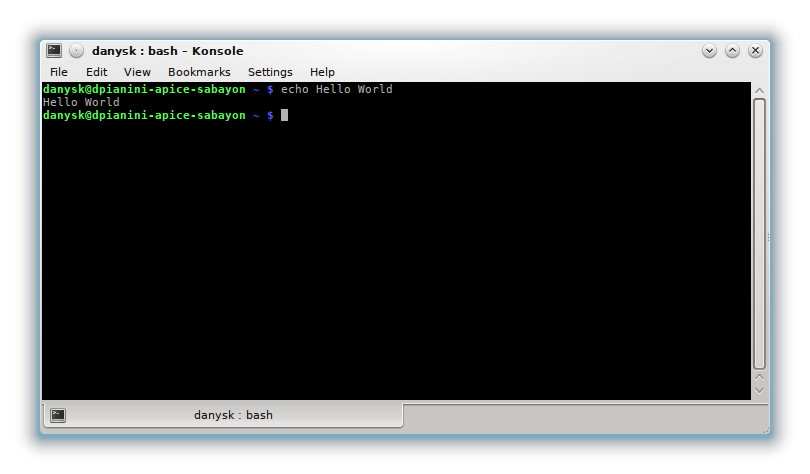
\includegraphics[width=0.99\columnwidth]{img/console}
\end{figure}
\end{frame}

\begin{frame}
\frametitle{...a così}
\begin{figure}
 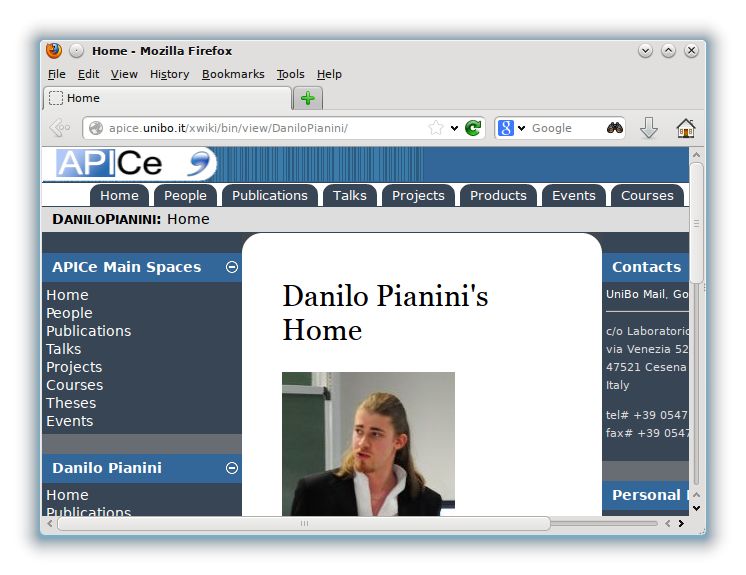
\includegraphics[width=0.99\columnwidth]{img/gui}
\end{figure}
\end{frame}

\section{Librerie per creare GUI}
\subsection{Astrazioni e struttura}

\begin{frame}
\frametitle{Librerie grafiche: quali astrazioni?}
Per creare interfacce grafiche, di norma, ci si appoggia a librerie esistenti
\begin{itemize}
 \item Avete visto in precedenza come sia possibile scrivere direttamente sul framebuffer, ma costruire un'applicazione dicendo ad ogni passo di che colore fare ciascun pixel è proibitivo
 \item Esistono librerie che vi forniscono strutture dati più vicine a quelle che volete realizzare, occupandosi loro del disegno su schermi
 \begin{itemize}
  \item Finestre
  \item Pulsanti
  \item Menu
  \item Caselle di testo
  \item e via dicendo
 \end{itemize}
\end{itemize}
\end{frame}

\begin{frame}
\frametitle{Librerie grafiche: come funzionano?}
Le librerie grafiche si appoggiano ad altre librerie, a scalare fino ai componenti che pilotano l'hardware video. 
Ogni volta che si sale di livello, le astrazioni si avvicinano sempre più a quelle che vorremmo usare per costruire interfacce.

\scriptsize
\centering
\begin{tabular}{| c | c | c |}
\hline & & \\
\textbf{Componente} & \textbf{Esempi} & \textbf{Astrazioni} \\
\hline & & \\
Libreria per GUI & GTK+, Qt, Swing & Pulsante, Layout, Area di testo... \\
\hline & & \\
Libreria per il disegno & GDK, AWT, Cairo & Colore, linea, punto, forma... \\
\hline & & \\
Compositor & Aqua, Compiz, Kwin, Aero & Decorazione, Effetto... \\
\hline & & \\
Server grafico & X, Quartz, Wayland & Schermo, finestra... \\
\hline & & \\
Kernel e drivers & Linux, Darwin & Dispositivo, Pixel... \\
\hline
\end{tabular}
\end{frame}

\subsection{Apprendere l'uso di nuove librerie}

\begin{frame}
\frametitle{Come imparare ad usare una libreria?}
Più che imparare \textbf{una} libreria delle tante, è meglio imparare \textbf{come si impara ad usare} una libreria che non si conosce.

Step da seguire:
\begin{enumerate}
 \item Quando possibile, cercare un documento che spieghi il genere di astrazioni che la libreria usa. Spesso, queste sono descritte brevemente nell'introduzione.
 \item Cercarsi un tutorial. Di norma, i migliori sono quelli scritti da chi ha creato la libreria.
 \item Seguire il tutorial, assicurandosi di capire la funzione di OGNI riga di codice, eventualmente commentando quelle non chiare per capire come cambia il comportamento del programma.
 \item Si riproducono gli esempi eventualmente arricchendoli, fin quando non si acquisisce manualità con lo strumento.
\end{enumerate}
\end{frame}

\section{GTK+3}

\subsection{Elementi generali}

\begin{frame}
\frametitle{GTK+3}
GTK+ (acronimo che sta per GIMP ToolKit) è un toolkit (insieme di strumenti) per la creazione di interfacce grafiche. Caratteristiche salienti:
\begin{itemize}
 \item Sviluppato in C
 \begin{itemize}
  \item Ma offre bindings anche per i linguaggi C++, Java, Python, Perl e Ruby
 \end{itemize}
 \item Multipiattaforma (anche se UNIX oriented)
 \item Software libero (parte del progetto GNU), licenza LGPL
 \item Molto diffuso
 \begin{itemize}
  \item GIMP, Firefox, Thunderbird, VMWare, Google Chrome e centinaia di altri software multi piattaforma usano GTK+
  \item Esistono interi ambienti grafici scritti in GTK+: GNOME, Mate, Xfce, LXDE...
 \end{itemize}
\end{itemize}
\end{frame}

\begin{frame}
\frametitle{E la concorrenza?}
Ovviamente esistono molte altre librerie. Abbiamo scelto di presentarvi GTK+ per i seguenti motivi:
\begin{itemize}
 \item Supporto al linguaggio C ``puro''
 \item Multipiattaforma
\end{itemize}

Di seguito, un breve elenco di librerie concorrenti.
\begin{itemize}
 \item Qt
 \begin{itemize}
  \footnotesize
  \item Principale concorrente di GTK+, altrettanto diffuso. Richiede conoscenze di Object Oriented Programming (OOP), che in questo corso non acquisite.
 \end{itemize}
 \item Swing
 \begin{itemize}
  \footnotesize
  \item Principale toolkit per interfacce grafiche in Java. Richiede conoscenze di OOP.
 \end{itemize}
 \item Windows Forms
 \begin{itemize}
  \footnotesize
  \item Create da Microsoft nella piattaforma .NET. Richiedono C\#.
 \end{itemize}
 \item Tk
 \begin{itemize}
  \footnotesize
  \item Come GTK+, ma più vecchio e meno diffuso.
 \end{itemize}
 \item Cocoa
 \begin{itemize}
  \footnotesize
  \item Solo per ambiente Apple Mac OSX, richiede Objective C.
 \end{itemize}
\end{itemize}
Ne esistono molti altri, i curiosi si dirigano su \url{http://en.wikipedia.org/wiki/List_of_widget_toolkits}
\end{frame}

\subsection{Elementi di base e compilazione}

\begin{frame}[fragile]
\frametitle{Compilazione di software GTK+}
\begin{itemize}
 \item Come per Glib, sfrutteremo \pkgconfig{} per compilare il nostro software
 \item GTK+ si appoggia a \textit{molte} altre librerie per poter funzionare: la compilazione senza l'aiuto di \pkgconfig{} è \textit{molto} dispendiosa
\end{itemize}
Output (su Linux, testato il \today{}) del comando:
\scriptsize
\begin{verbatim}
pkg-config --cflags --libs gtk+-3.0
\end{verbatim}
\scriptsize
\begin{verbatim}
-pthread -I/usr/include/gtk-3.0 -I/usr/include/at-spi2-atk/2.0
-I/usr/include/at-spi-2.0 -I/usr/include/dbus-1.0 -I/usr/lib/dbus-1.0/include
-I/usr/include/gtk-3.0 -I/usr/include/gio-unix-2.0/ -I/usr/include/cairo
-I/usr/include/pango-1.0 -I/usr/include/atk-1.0 -I/usr/include/cairo
-I/usr/include/pixman-1 -I/usr/include/freetype2 -I/usr/include/libpng16
-I/usr/include/harfbuzz -I/usr/include/freetype2 -I/usr/include/harfbuzz
-I/usr/include/libdrm -I/usr/include/libpng16 -I/usr/include/gdk-pixbuf-2.0
-I/usr/include/libpng16 -I/usr/include/glib-2.0 -I/usr/lib/glib-2.0/include
-lgtk-3 -lgdk-3 -lpangocairo-1.0 -lpango-1.0 -latk-1.0 -lcairo-gobject -lcairo
-lgdk_pixbuf-2.0 -lgio-2.0 -lgobject-2.0 -lglib-2.0
\end{verbatim}
\normalsize
Scrivere ogni volta una cosa così a mano è fuori questione.
\end{frame}


\begin{frame}[fragile]
\frametitle{Primo esempio con GTK+3}
\scriptsize
\begin{lstlisting}[language=C]
#include <gtk/gtk.h>

static void activate(GtkApplication *app, gpointer user_data) {

   // In GTK+ ogni cosa (finestre, pulsanti...) e' un widget 
   GtkWidget *window = gtk_application_window_new(app);

   // Mostra a schermo questo widget e tutti quelli in esso contenuti
   gtk_widget_show_all(window);
}

int main(int argc, char **argv) {
   // Dichiara una nuova applicazione
   GtkApplication *app;
   int status;

   // Crea una nuova applicazione
   app = gtk_application_new("it.unibo.EmptyWindow", G_APPLICATION_FLAGS_NONE);

   // Quando l'applicazione viene attivata, esegui la funzione "activate"
   g_signal_connect(app, "activate", G_CALLBACK(activate), NULL);
   
   // Esegue l'applicazione. Il controllo passa a GTK+
   status = g_application_run(G_APPLICATION(app), 0, NULL );
   g_object_unref(app);
   return status;
}
\end{lstlisting} 
\end{frame}

\begin{frame}
\frametitle{Risultato}
\begin{figure}
 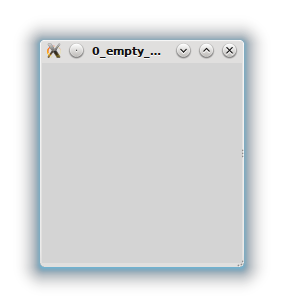
\includegraphics[width=0.6\columnwidth]{img/0}
\end{figure}
\end{frame}

\subsection{Pulsanti}

\begin{frame}[fragile]
\frametitle{Un pulsante in GTK+3}
\begin{lstlisting}[language=C]
#include <gtk/gtk.h>

static void activate(GtkApplication *app, gpointer user_data) {
   // Anche il pulsante è un GtkWidget!
   GtkWidget *window, *button;
   window = gtk_application_window_new(app);
   gtk_window_set_title(GTK_WINDOW (window), "A button");

   // Questa funzione crea un nuovo GtkButton e ne torna il puntatore
   button = gtk_button_new_with_label("This is a button");
   
   // Questa funzione consente di aggiungere il pulsante alla finestra
   gtk_container_add (GTK_CONTAINER (window), button);
   gtk_widget_show_all(window);
}

int main(int argc, char **argv) {
   GtkApplication *app;
   int status;
   app = gtk_application_new("it.unibo.EmptyWindow", G_APPLICATION_FLAGS_NONE);
   g_signal_connect(app, "activate", G_CALLBACK(activate), NULL);
   status = g_application_run(G_APPLICATION(app), 0, NULL );
   g_object_unref(app);
   return status;
}
\end{lstlisting} 

\end{frame}

\begin{frame}
\frametitle{Risultato}
\begin{figure}
 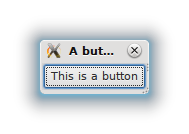
\includegraphics[width=0.6\columnwidth]{img/2}
\end{figure}
\end{frame}


\subsection{Eventi}

\begin{frame}
\frametitle{Gestione degli eventi}
Cosa accade quando viene premuto il nostro pulsante?
\begin{itemize}
 \item Assolutamente nulla.
\end{itemize}
Perché?
\begin{itemize}
 \item Non abbiamo scritto da nessuna parte che cosa deve succedere a fronte della pressione del pulsante.
\end{itemize}
Descrivere che cosa debba accadere a fronte delle azioni che vengono compiute da chi interagisce con il software prende il nome di ``gestione degli eventi''.
\end{frame}

\begin{frame}
\frametitle{Signals e Callbacks}
Diverse librerie hanno modelli di gestione diversa degli eventi, GTK+3 usa i segnali e le callbacks
 \begin{itemize}
  \item Ciascun componente ha un insieme di ``signal''
  \begin{itemize}
   \item Ad esempio i pulsanti hanno disponibili i signal ``activate'', ``clicked'', ``enter'', ``leave'', ``pressed'' e ``released''.
  \end{itemize}
  \item È possibile associare a ciascuno di questi signal una ``callback'', ossia una funzione con una particolare signature
  \item Ogni volta che accade un evento riguardante quel componente, viene generato il signal corrispondente
  \item A fronte della generazione del signal, tutte le callback ad esso associato vengono eseguite
 \end{itemize}
Ad esempio, potremmo fare in modo che il nostro pulsante stampi a video qualcosa quando premuto.
\end{frame}

\begin{frame}[fragile]
\frametitle{Un pulsante \textbf{funzionante} in GTK+3}
\begin{lstlisting}[language=C]
#include <gtk/gtk.h>

// Questa e' una callback. In questo caso, gli argomenti passati
// non vengono utilizzati
static void print_hello(GtkWidget *widget, gpointer data) {
   printf("Hello World\n");
}

static void activate(GtkApplication *app, gpointer user_data) {
   GtkWidget *window, *button;
   window = gtk_application_window_new(app);
   gtk_window_set_title(GTK_WINDOW (window), "A button");
   button = gtk_button_new_with_label("This is a button");
   gtk_container_add(GTK_CONTAINER (window), button);

   /* Associa la callback "print_hello" al segnale "clicked"
    * Notare che "G_CALLBACK (&print_hello)" e' ASSOLUTAMENTE IDENTICO
    * a G_CALLBACK (print_hello).
    */
   g_signal_connect(button, "clicked", G_CALLBACK (print_hello), NULL);
   gtk_widget_show_all(window);
}

int main(int argc, char **argv) {
   [...vedi prima...]
}
\end{lstlisting}
\end{frame}

\begin{frame}
\frametitle{Risultato}
\begin{figure}
 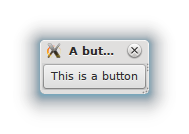
\includegraphics[width=0.6\columnwidth]{img/3}
\end{figure}
\end{frame}

\begin{frame}[fragile]
\frametitle{Un altro pulsante \textbf{funzionante} in GTK+3}
\begin{lstlisting}[language=C]
#include <gtk/gtk.h>

// Dichiaro globale il pulsante, per poterlo usare ovunque
GtkWidget *button;

// Quante callbacks! Cambio l'etichetta del pulsante a seconda dell'evento
static void pressed(GtkWidget *widget, gpointer data) {
   gtk_button_set_label(GTK_BUTTON(button), "Pressed");
}
static void released(GtkWidget *widget, gpointer data) {
   gtk_button_set_label(GTK_BUTTON(button), "Released");
}
static void enter(GtkWidget *widget, gpointer data) {
   gtk_button_set_label(GTK_BUTTON(button), "Mouse Entered");
}
static void leave(GtkWidget *widget, gpointer data) {
   gtk_button_set_label(GTK_BUTTON(button), "Mouse Left");
}

static void activate(GtkApplication *app, gpointer user_data) {
   [...vedi prima...]

   // Molti signals molto onore
   g_signal_connect(button, "enter", G_CALLBACK (enter), NULL);
   g_signal_connect(button, "leave", G_CALLBACK (leave), NULL);
   g_signal_connect(button, "pressed", G_CALLBACK (pressed), NULL);
   g_signal_connect(button, "released", G_CALLBACK (released), NULL);
   gtk_widget_show_all(window);
}

int main(int argc, char **argv) {
   [...vedi prima...]
}
\end{lstlisting}
\end{frame}

\begin{frame}
\frametitle{Risultato}
\begin{figure}
 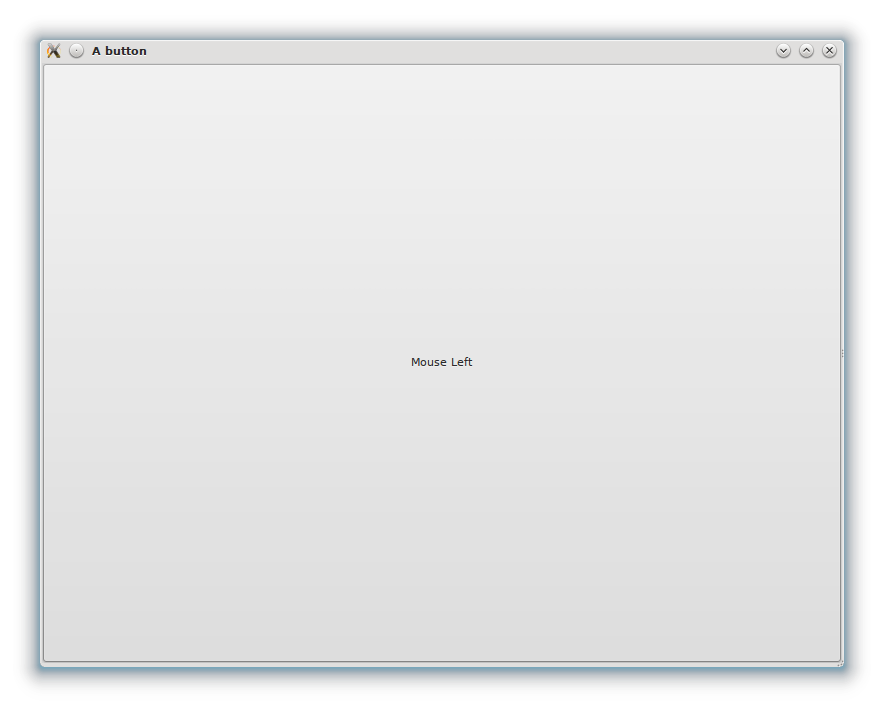
\includegraphics[width=0.99\columnwidth]{img/4}
\end{figure}
\end{frame}

\subsection{Altri componenti}

\begin{frame}
\frametitle{Altri componenti}
GTK+3 supporta molti altri tipi di componenti oltre ai pulsanti. Non riusciremo a sviscerarli nel poco tempo a disposizione oggi, di seguito avete un elenco \textbf{molto} parziale. Descrizioni migliori sono presenti alle pagine linkate.
\begin{itemize}
 \scriptsize
 \item Pulsanti \url{https://developer.gnome.org/gtk3/3.2/ButtonWidgets.html}
 \begin{itemize}
 \tiny
  \item GtkButton (generano un segnale quando si clickano)
  \item GtkCheckButton (selettore discreto)
  \item GtkRadioButton (scelta multipla)
 \end{itemize}
 \scriptsize
 \item Testo \url{https://developer.gnome.org/gtk3/3.2/NumericEntry.html}
 \begin{itemize}
 \tiny
  \item GtkEntry (campo di testo modificabile a singola linea)
  \item GtkScale (slitta che consente di scegliere un valore in una range predefinito)
  \item GtkSpinButton (campo di testo a singola linea per valori numerici, con pulsanti)
  \item GtkEditable (area di testo multi-linea)
 \end{itemize}
 \scriptsize
 \item Menu \url{https://developer.gnome.org/gtk3/3.2/MenusAndCombos.html}
 \begin{itemize}
 \tiny
  \item GtkComboBox (menu a tendina con selezione multipla)
  \item GtkMenuBar (classico menu posizionato in alto nelle finestre)
  \item GtkMenuItem  (elemento di un menu)
 \end{itemize}
 \scriptsize
 \item Selettori \url{https://developer.gnome.org/gtk3/3.2/SelectorWidgets.html}
 \begin{itemize}
 \tiny
  \item GtkFileChooser (classica finestra per apri/salva file)
  \item GtkFontChooser (consente di selezionare tipo e dimensione del testo)
  \item GtkColorButton (pulsante che lancia una selezione di colore)
  \item GtkHSV (ruota di colori)
 \end{itemize}
 \scriptsize
 \item Scrolling \url{https://developer.gnome.org/gtk3/3.2/ScrollingWidgets.html}
 \begin{itemize}
 \tiny
  \item GtkScrollbar (classica barra di scorrimento)
 \end{itemize}
\end{itemize}

\end{frame}

\begin{frame}
\frametitle{Componenti personalizzati}
\begin{itemize}
 \item Nonostante la libreria GTK+3 sia molto ricca, esiste sempre l'eventualità che si voglia un nuovo componente
 \item È possibile crearsi nuovi componenti specificando il modo in cui essi devono essere disegnati
 \item Per disegnare GTK+3 si appoggia alla libreria Cairo
 \item A sua volta Cairo utilizza GDK
 \item Si tratta, sostanzialmente, di descrivere come una penna dovrebbe muoversi in una griglia per delineare i contorni di ciò che vogliamo disegnare, quindi scegliere un colore, ed infine scegliere se riempire o solo disegnare il contorno.
\end{itemize}
\end{frame}

\begin{frame}[fragile]
\frametitle{I colori, \texttt{colorfactory.h}}
Uno degli elementi necessari a disegnare sono i colori. GTK+ si appoggia a GDK, che contiene strutture dati per rappresentare i colori. Per semplificare ulteriormente, useremo una libreria personalizzata per gestire quattro colori (nero, bianco, rosso, blu).
\begin{lstlisting}[language=C]
#ifndef COLORFACTORY_H_
#define COLORFACTORY_H_

const GdkRGBA* color_white;
const GdkRGBA* color_black;
const GdkRGBA* color_blue;
const GdkRGBA* color_red;

void init_color_factory(void);

#endif /* COLORFACTORY_H_ */
\end{lstlisting}
\end{frame}

\begin{frame}[fragile]
\frametitle{I colori, \texttt{colorfactory.c}}
\begin{lstlisting}[language=C]
#include <gtk/gtk.h>
#include "colorfactory.h"

static GdkRGBA* gen_color_white(void) {
   GdkRGBA *white = (GdkRGBA *) malloc(sizeof(GdkRGBA));
   white->red = 1.0;
   white->green = 1.0;
   white->blue = 1.0;
   white->alpha = 1.0;
   return white;
}

[altre funzioni gen_color_*(void) qui]

void init_color_factory(void) {
   color_white = gen_color_white();
   color_black = gen_color_black();
   color_blue = gen_color_blue();
   color_red = gen_color_red();
}
\end{lstlisting}
\end{frame}

\begin{frame}[fragile]
\frametitle{Area di disegno}
\begin{lstlisting}[language=C]
#include <gtk/gtk.h>
// Usiamo anche la nuova libreria con i colori
#include "colorfactory.h"

// Dichiariamo un widget che sara' un'area di disegno
GtkWidget *drawing_area;

gboolean draw(GtkWidget *widget, cairo_t *cr, gpointer data) {
   [implementazione nella prossima slide]
}

static void activate(GtkApplication *app, gpointer user_data) {
   GtkWidget *window;
   window = gtk_application_window_new(app);
   gtk_window_set_title(GTK_WINDOW (window), "Drawing area");
   gtk_window_set_default_size(GTK_WINDOW(window), 800, 600);
   
   // Creazione dell'area di disegno
   drawing_area = gtk_drawing_area_new();
   gtk_widget_set_size_request(drawing_area, 500, 500);
   
   // Associazione della callback di disegno al segnale "draw"
   g_signal_connect(G_OBJECT(drawing_area),"draw",G_CALLBACK (draw),NULL);
   
   gtk_container_add(GTK_CONTAINER (window), drawing_area);
   gtk_widget_show_all(window);
}

int main(int argc, char **argv) {
   [come prima]
}
\end{lstlisting}
\end{frame}

\begin{frame}[fragile]
\frametitle{Area di disegno}
\begin{lstlisting}[language=C]
gboolean draw(GtkWidget *widget, cairo_t *cr, gpointer data) {

   // calcolo larghezza e altezza, e il maggiore dei due
   const int width = gtk_widget_get_allocated_width(widget);
   const int height = gtk_widget_get_allocated_height(widget);
   const int max = width > height ? height : width;
   
   // Disegno lo sfondo: un rettangolo...
   cairo_rectangle(cr, 0, 0, width, height);
   // ...bianco...
   gdk_cairo_set_source_rgba(cr, color_white);
   // ...pieno (non disegno solo i contorni ma lo riempio)
   cairo_fill(cr);

   // Disegno un cerchio nero
   cairo_arc(cr,width/2,height/2, max / 3, 0 , 360.0);
   gdk_cairo_set_source_rgba(cr, color_black);
   cairo_fill(cr);

   // Ora disegno una circonferenza blu
   cairo_arc(cr,width/2,height/2, max / 2.5, 0 , 360.0);
   gdk_cairo_set_source_rgba(cr, color_blue);
   cairo_stroke(cr);

   return FALSE;
}

\end{lstlisting}
\end{frame}

\begin{frame}
\frametitle{Risultato}
\begin{figure}
 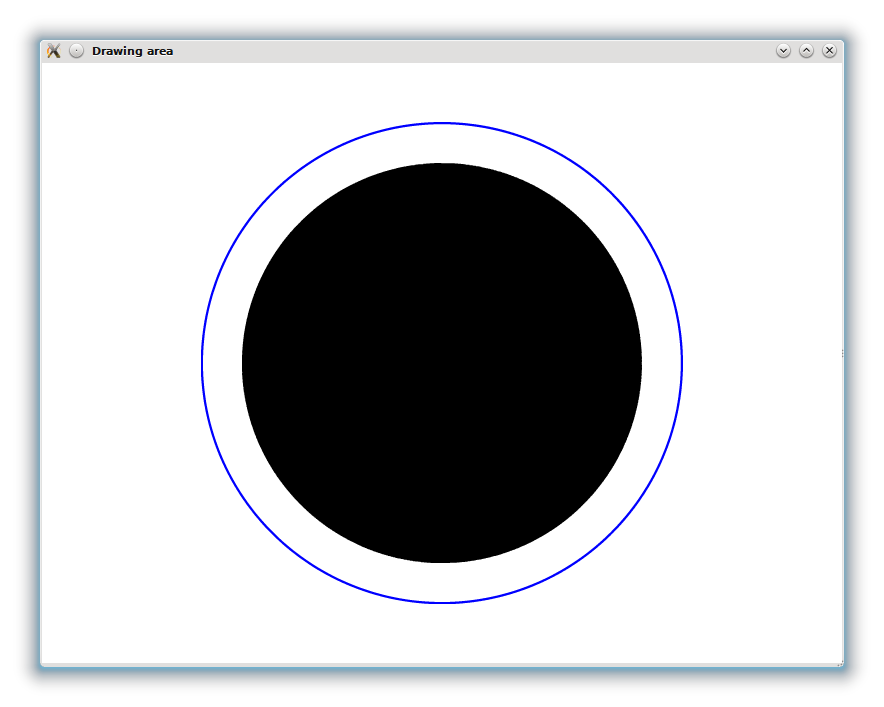
\includegraphics[width=0.99\columnwidth]{img/5}
\end{figure}
\end{frame}

\subsection{Container e layout}
\begin{frame}
\frametitle{Container}
\begin{itemize}
 \item Finora abbiamo solo utilizzato un componente alla volta, ma di norma se ne usa più d'uno.
 \item Per aggiungere più di un componente alla stessa finestra, occorre utilizzare un ``container''
 \item Il container è uno speciale Widget che ha come scopo quello di contenere altri widget
  \begin{itemize}
   \item ...inclusi altri container
   \item Come in un gioco di scatole cinesi
  \end{itemize}
 \item Vedremo l'uso del BoxLayout
  \begin{itemize}
   \item È uno dei più semplici
   \item Utilizzandolo correttamente si possono ottenere moltissime organizzazioni dei componenti
  \end{itemize}
\end{itemize}
\end{frame}

\begin{frame}[fragile]
\frametitle{Pulsante che controlla l'area di disegno}
\begin{lstlisting}[language=C]
#include <gtk/gtk.h>
#include "colorfactory.h"

// Useremo un pulsante ed un'area di disegno
GtkWidget *button, *drawing_area;
// Questo token vale TRUE se si vuole disegnare un cerchio, false altrimenti
int draw_circle = TRUE;

// Funzione che decide quale etichetta mettere al pulsante
static char *getLabel(void) {
   return draw_circle ? "Click to draw a square" : "Click to draw a circle";
}

// Evento da eseguire a seguito del click sul bottone
static void clicked(GtkWidget *widget, gpointer data) {
   // Se disegna il contrario di quel che disegnavi prima
   draw_circle = !draw_circle;
   // setta la corretta etichetta
   gtk_button_set_label(GTK_BUTTON(button), getLabel());
   // Forza un ridisegno di tutta la finestra
   gtk_widget_queue_draw_area(GTK_WIDGET(drawing_area), 0, 0, 5000, 5000);
}
\end{lstlisting}
\end{frame}

\begin{frame}[fragile]
\frametitle{Pulsante che controlla l'area di disegno}
\begin{lstlisting}[language=C]
gboolean draw(GtkWidget *widget, cairo_t *cr, gpointer data) {
   int width = gtk_widget_get_allocated_width(widget);
   int height = gtk_widget_get_allocated_height(widget);
   int max =  (width > height ? height : width);
   cairo_rectangle(cr, 0, 0, width, height);
   gdk_cairo_set_source_rgba(cr, color_white);
   cairo_fill(cr);
   
   // Se devi disegnare un cerchio fai un cerchio, altrimenti un rettangolo
   if (draw_circle) {
      cairo_arc(cr, width / 2, height / 2, max / 3, 0, 360.0);
   } else {
      cairo_rectangle(cr, width / 4, height / 4, width / 2, height / 2);
   }
   gdk_cairo_set_source_rgba(cr, color_black);
   cairo_fill(cr);
   return FALSE;
}
\end{lstlisting}
\end{frame}


\begin{frame}[fragile]
\frametitle{Pulsante che controlla l'area di disegno}
\begin{lstlisting}[language=C]
static void activate(GtkApplication *app, gpointer user_data) {
   GtkWidget *window, *layout;
   window = gtk_application_window_new(app);
   gtk_window_set_title(GTK_WINDOW (window), "Drawing area");
   gtk_window_set_default_size(GTK_WINDOW(window), 800, 500);

   // Crea l'area di disegno e associa la callback corrispondente
   drawing_area = gtk_drawing_area_new();
   gtk_widget_set_size_request(drawing_area, 500, 500);
   g_signal_connect(G_OBJECT (drawing_area), "draw", G_CALLBACK (draw), NULL);

   // Crea il bottone e associa la callback all'evento di click
   button = gtk_button_new_with_label(getLabel());
   g_signal_connect(button, "clicked", G_CALLBACK (clicked), NULL);

   // Crea un BoxLayout verticale
   layout = gtk_box_new(GTK_ORIENTATION_VERTICAL, 5);
   
   // Mettici dentro prima il bottone, quindi l'area di disegno
   gtk_container_add(GTK_CONTAINER (layout), button);
   gtk_container_add(GTK_CONTAINER (layout), drawing_area);
   
   // Inserisci il container nella finestra
   gtk_container_add(GTK_CONTAINER (window), layout);

   // Mostra la finestra
   gtk_widget_show_all(window);

}

int main(int argc, char **argv) {
   [solito main sempre uguale]
}
\end{lstlisting}
\end{frame}

\begin{frame}
\frametitle{Risultato}
\begin{figure}
 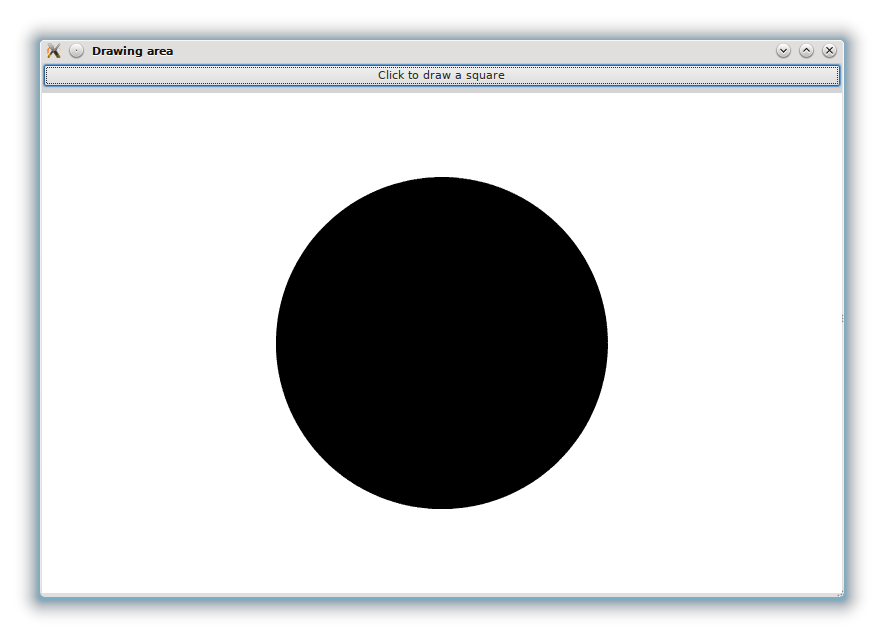
\includegraphics[width=0.99\columnwidth]{img/6}
\end{figure}
\end{frame}


\section{Nell'ultimo laboratorio: un'applicazione completa}

\begin{frame}
\frametitle{Un'applicazione completa in C}
\begin{itemize}
 \item Ho realizzato una semplice applicazione C in grado di disegnare su schermo alcune funzioni matematiche
 \item In laboratorio la modificheremo aggiungendo delle nuove funzionalità
\begin{figure}
 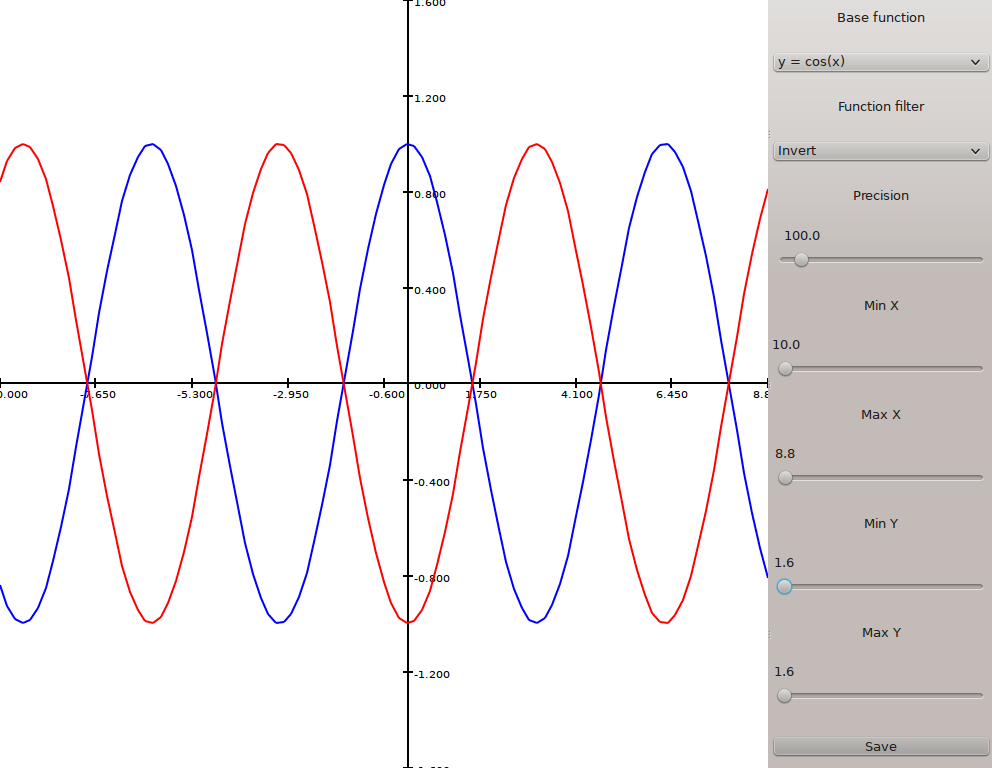
\includegraphics[width=0.5\columnwidth]{img/fd}
\end{figure}
\end{itemize}
\end{frame}

% \begin{frame}
% \frametitle{Organizzazione logica}
% Dalle funzionalità estrapolare i componenti. Divide et impera
% \end{frame}
% 
% \begin{frame}
% \frametitle{Descrizione dell'applicazione}
% GUI e funzionalità
% \end{frame}

\end{document}

